\iffalse
\bibliography{myreference.bib}
\fi
%chapter 2 feature analysis

\chapter{Feature Analysis}
\section{Feature}
A feature is an individual measurable property of a phenomenon being observed\cite{bishop2006pattern}. It is an important part of an observation or a sample for learning about the structure of the problem that is being modeled.
\begin{figure}[h]\centering 
\begin{subfigure}[b]{0.4\textwidth} 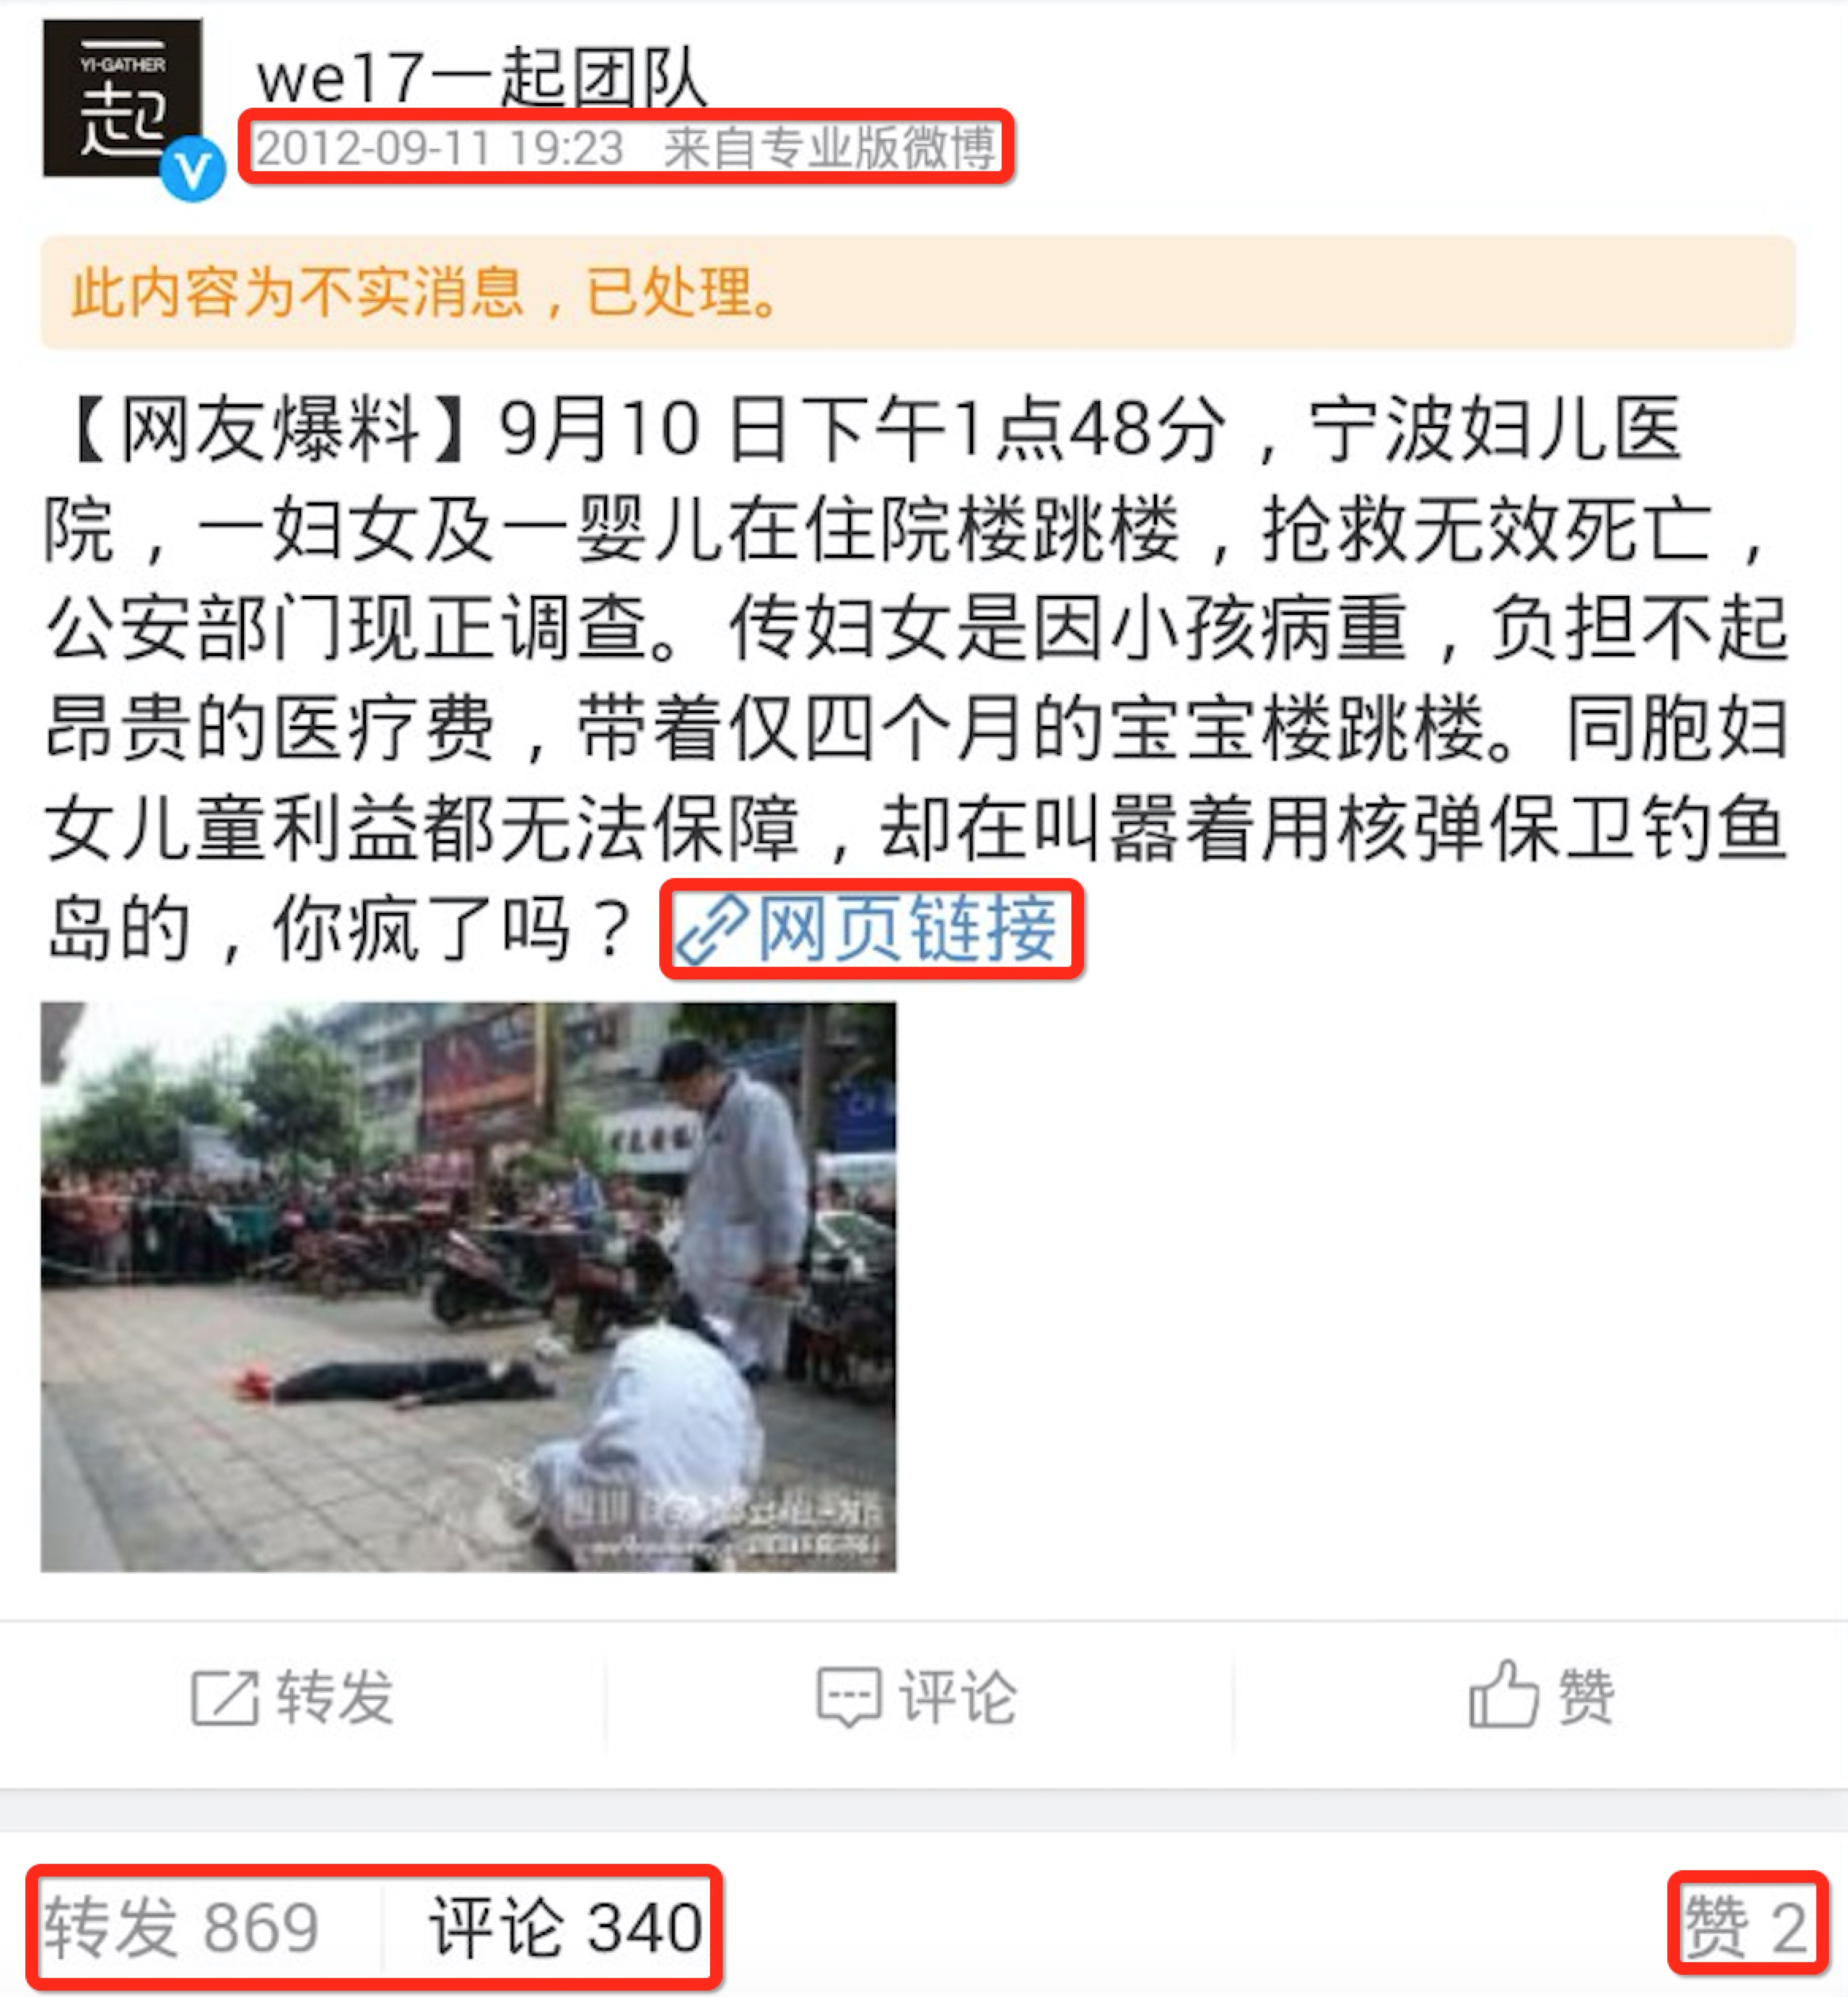
\includegraphics[width=55mm, height=65mm]{feature1} \caption{Feature of Weibo} \label{fig:Weibo} \end{subfigure} \qquad \qquad
\begin{subfigure}[b]{0.4\textwidth} 
\includegraphics[width=55mm, height=65mm]{feature2} \caption{Feature of User} \label{fig:User} \end{subfigure}
\caption{Features}\label{fig:features} \end{figure}

In this project, some features we are dealing with are circumscribed shown in Fig. \ref{fig:features}. This is an original rumor-related Weibo along with its author. This message has 869 reposts and 340 comments with 2 likes in the left figure. The author also has some features about the number of friends, followers and Weibo he or she has. These features are called explicit features, which means we can simply acquire them without further processing. Another kind of feature is called implicit feature that needs to be extracted. We discuss this part in the next section.

\section{Feature Extraction}
Feature extraction is an important step before training a model. It is a process of building derived features inside the data. Feature extraction reduces the useless information while retains the necessary resource to describe a large set of data. By doing this part, we don't need a large amount of memory to store those variables and large computation power to train the model with the risk of overfitting the training samples. The extracted features are expected to contain the related information from the input data.

Castillo et al. extract four types of features including message-based feature, user-based feature, topic-based feature and propagation-based feature\cite{castillo2011information}. Similarly, Qazvinian et al. use content-based features, network-based features and Twitter Specific memes\cite{qazvinian2011rumor}. For the first one, they present the tweet with lexical patterns and part-of-speech patterns\cite{hassan2010s}. In the network-based features, they use two types of log-likelihood ratio feature to capture four tpyes of network-based properties. For the Twitter specific memes, they use hashtags and URLs, which has shown the usefulness in \cite{ratkiewicz2010detecting}.

For researching in Sina Weibo, besides the previous feature,  Wu et al. also extract the propagation feature towards the transmission path of Weibo\cite{wu2015false}. Yang et al. propose two new feature, the location of event and the client program used for posting the microblog.\cite{yang2012automatic} Later in the experiment part, we will discuss the feature we extract and its method.

\section{Feature Selection}
After doing the feature extraction, many features are acquired. However, some features are irrelevant to the problem. There are some features that will be more important than others to the model. Also, some features may be redundant in the context of other features. The focus of feature selection is to select a subset of feature, which can efficiently represent the input data, from the original input feature vector for reducing effects from noise or irrelevant features while still has a good classification or prediction result of the model trained by the chosen features\cite{guyon2003introduction}. Thus it is helpful to do feature selection. Feature selection can reduce the number of attributes in the dataset, which is quite similar to the dimensionality reduction. But they are different. For the dimensionality reduction, it reduces the number of features by creating new combinations of attributes such as Principal Component Analysis\cite{jolliffe2002principal} and Singular Value Decomposition\cite{de1994singular}, while feature selection only choose the attributes present in the data without changing them.

Feature selection method can be divided into three types including filer methods, wrapper methods and embedded methods.
\subsection{Filter methods}
Filter methods are applied before training a model. These methods need quantitative criteria to measure the relevance of each feature with the output class. Then these features can be ranked by the value of criteria and be selected by ordering. It is helpful in the practical application due to the simplicity computation. Usually, a threshold is needed to decide whether a feature can be retained or not. 

Next we will discuss how to measure the relevance of a feature to the output.

\subsubsection{Pearson product-moment correlation coefficient}

One of the simplest criteria is the Pearson correlation coefficient\cite{benesty2009pearson}.
\begin{equation} \label{Eq:pearsoncoefficient}
R(i)=\frac{cov(x_i,Y)}{\sqrt{var(x_i)*var(Y)}}
\end{equation}
where $x_i$ vector is the $i_{th}$ sample. Y is the output class. $cov()$ is the covariance of $x_i$ and $Y$ and $var()$ is the variance of the variable. This method can detect the linear correlation between variable $x_i$ and the target. The value of this coefficient is in the range of -1 to +1, where +1 is total positive correlation, 0 is no correlation and -1 represents the total negative correlation. However, only the numerical or continuous type data can use it.
\subsubsection{Mutual Information}
Shannon's information theory\cite{shannon2001mathematical} tolds us the method to quantify the \textit{entropy} by the following equation:
\begin{equation} \label{Eq:entropy}
H(C)=-\sum_{c=1}^{N_c}{P(c)\log(P(c))}
\end{equation}
where $P(c)$ is the probability for the different classes. $c=1,...N_c$. This equation represents the uncertainty in the output class. If we know the feature vector $\bm{f}$, the \textit{conditional entropy} is:
\begin{equation} \label{Eq:conditionalEntropy}
H(C|F)=-\sum_{f=1}^{N_f}{P(\bm{f})(\sum_{c=1}^{N_c}{P(c|\bm{f})\log{P(c|\bm{f})})}}
\end{equation}
where $P(c|\bm{f})$ is the conditional probability for class c given the input feature vector $\bm{f}$

If the input feature vector is of continuous variable, we need to do an integral. The probabilities will be replaced by the probability densities, like the following equation:
\begin{equation} \label{Eq:continuousEntropy}
H(F) = -\int{P(f)\log{P(f)}}df
\end{equation}
In general, the conditional entropy will be less than the initial entropy, except the situation that if and only if the feature is completely independent to the output class. For example, if the joint probability density is equal to the product of the probability density of this feature and the class. Thus comes to the definition of \textit{mutual information}:
\begin{equation} \label{Eq:MutualInformaion}
I(C;F)=H(C)-H(C|F)
\end{equation}
It is a symmetric to the C and F. It can also be expressed by the following equation:
\begin{equation} \label{Eq:MutualInformaionDiscrete}
I(C;F)=\sum_{c,\bm{f}}{P(c,\bm{f})\log{\frac{P(c,\bm{f})}{P(c)P(\bm{f})}}}
\end{equation}
or by the continuous feature version of mutual information:
\begin{equation} \label{Eq:MutualInformaionContinuous}
I(C;F)=\sum_c{\int{P(c,\bm{f})\log{\frac{P(c,\bm{f})}{P(c)P(\bm{f})}}}d\bm{f}}
\end{equation}
We use $\bm{f}$ rather than one specific feature as the input. Actually, if we want to find out whether one feature has dependence with the output, we can simply calculate the mutual information by the following equation:
\begin{equation} \label{Eq:MutualInformaionDiscrete}
I(X;Y)=\sum_{y\in{Y}}{\sum_{x\in{X}}{p(x,y)\log{\frac{p(x,y)}{p(x)p(y)}}}}
\end{equation}
These equation above show that if X and Y are independent then the value of mutual information would be zero. The dependent feature can decrease the uncertainty by providing information to the class\cite{battiti1994using}.

The filter methods don't rely on learning algorithm so that they are not very computation comsuming. However, these methods may not perform well when there are redundant features in the input feature vector because filer methods only calculate the relevance between output class and feature one by one. Under this circumstance, the ``optimal'' subset selected by filter methods may contain many highly-correlated features. However, even if one feature has less information to the output class by its own, but may be informative when combined with other features\cite{xu2010discriminative}.
\subsection{Wrapper methods}
Wrapper methods is done using the induction algorithm as a black box and use the predictor or classifier performance, usually the accuracy of model, as the objective function to evaluate the feature subset\cite{kohavi1997wrappers}. Suppose we have $N$ features, we will need to evaluate $2^N$ subset of features, which is a NP-hard problem. If we just evaluate the whole space exhaustively, it will be very computation consuming. To solve this problem, several methods are proposed.
\subsubsection{Sequential selection algorithms}
These methods start with an empty set and iteratively add one feature into the feature subset. Each time it selects the feature from the remaining features that can give the highest value for the objective function. This process is terminated once the required number of feature is added. On the opposite direction, we can also start with a full set and remove one feature each step which that gives the lowest decrease on the value of objective function. These two method, called Sequential Feature Selection (SFS) and Sequential Backward Selection (SBS), are naive search algorithm because it doesn't take the dependency between features into account. 

Pudil et al. do a little improvement on the naive version of SFS, call Sequential Float Feature Selection (SFFS). They introduce an additional step called backtracking step. After a feature is added into the subset, they try to reach a better performance of the objective function by removing one feature from it\cite{pudil1994floating}. If the performance is getting better, they use the reduced subset to do this trial again until no more performance increase. Then do the feature addition as usual.

On the basis of SFFS, some researchers propose further improvement. Nakariyakul and Casasent add an additional search step called ``replacing the weak feature'' to check whether removing any feature in the current selected subset and adding a new one at each sequential step can improve the performance of current feature subset\cite{nakariyakul2009improvement}. They provide the optimal or quasi-optimal solution for many selected subsets. This solution requires significantly less computation than the optimal feature selection algorithm.

\subsubsection{Heuristic search algorithms}
When $N$ is relatively large, heuristic search methods such as genetic algorithm\cite{golberg1989genetic} can be used to reduce the computation load. It uses the chromosome bits to represent whether a feature is included in the subset or not. If a bit is 1, it means that the corresponding feature is selected while 0 means the corresponding feature is not selected. A typical run of genetic algorithm involves many generations, or we can say the iteration. In each iteration, evaluation of an individual chromosome, which represents a specific subset of feature, involves training a model and compute the accuracy. In genetic algorithm, there are several parameter that can be tuned as followed:
\begin{enumerate} \item Population size \item Number of generations \item Probability of crossover \item Probability of mutation \item Probability of selection of the highest ranked individual
\end{enumerate}
These concept can be found in this link\footnote{\url{https://en.wikipedia.org/wiki/Genetic_algorithm}}.
Yang and Honavar implement this heuristic search algorithm to do feature selection\cite{yang1998feature}. To evaluate the individual chromosome, in genetic algorithm called fitness, they use neural network trained by DistAl\cite{yang1998distal} and evaluate the performance of it by accuracy. Besides, they also calculate the cost of performing the classification. Thus the fitness of chromosome can be represented as the following equation:
\begin{equation} \label{Eq.fitness}
fitness(x)=accuracy(x)-\frac{cost(x)}{accuracy(x)+1}+cost_{max}
\end{equation}
where $x$ is a subset of features and $accuracy(x)$ is the test accuracy of the neural-network classifier using the subset feature $x$. $cost(x)$ is the sum of measurement costs of the feature subset $x$. By choosing the largest value of $fitness(x)$, its corresponding subset of feature are considered as the optimal selection result.

The obvious drawback of wrapper methods is that for each subset of feature, a model is needed to be trained. So the execution time of algorithms will be very long when the number of sample and feature is large. Also, for genetic algorithm, same subset of feature may be repeatedly evaluated. Overfitting is an another drawback if the model learns the data too well.

\subsection{Embedded methods}
Since we have so many drawbacks to the filter and wrapper methods we discussed above, the embedded methods try to reduce the bad influence to the feature selection. The principle of these methods is that when doing the training process, the task of feature selection is done simultaneously.

The most popular methods involves:
\begin{enumerate} \item $l_1$-norm or $l_2$-norm regularization linear model like LASSO or $l_1$-SVM \item Decision tree model \item SVM with Recursive Feature Elimination
\end{enumerate}
Since all of them are used in this project, the concept of them will be discussed later.
\section{Feature Importance}
After feature extraction and feature selection, we roughly acquire the scores allocating for the features. They can also be ranked by their scores. However, the score may be calculated by different method or represented by different coefficient, thus the comparison of value of the score between different method is meaningless. Features importance can provide us a intuitively feeling towards the problem. Meanwhile, by using the features with high score, we can construct new features. In this project, we want to find the most important features that can help us to train a better model for classifying whether a Weibo is a rumor or not.
\section{Benefit of Feature Analysis}
What feature analysis can achieve is that we can use less but more important features to train models rather than input a high dimensional feature vector. If the data is in a high dimension, the curse of dimensionality will occurs. Data becomes increasingly sparse in the space. The density and distance between each sample increase so that data becomes dissimilar which prevents algorithm from finding the inside structure or relation. For example, some algorithms based on calculating the distance to find similar samples, like $k$-nearest neighbors algorithm\cite{altman1992introduction} or $k$-means clustering\cite{hartigan1979algorithm}, become less meaningful. Also, anomaly detection may face some problems because all of the distances become numerically similar\cite{zimek2012survey}.

Actually, when training models, the computation time and required memory will exponentially increase as the dimention of data increases. Meanwhile, even if the models can be trained, the complexity of model will be too complex, which will cause the \textit{deterministic noise}\cite{abu2012learning}. The overfitting will occurs because the models try to fit the noise either the stochastic noise or the deterministic noise.
